%-------------------------
% Rover Resume - Star Template
% Link: https://github.com/subidit/rover-resume
%
% CUSTOM COMMANDS \aux{} and \rside{} for part formatting
% eg. \subsection{Company Name \aux{Designation} \rside{Duration}}
% Double lined titles with \subsection{} and \subsubsection{}
% \linkicon gives external link icon
%-------------------------

\documentclass[11pt]{article}
\usepackage[T1]{fontenc}
\usepackage[utf8]{inputenc}

\usepackage[sfdefault,semibold,lf]{FiraSans}
\usepackage[a4paper,margin=1in]{geometry}

\usepackage{xcolor}
\definecolor{accent}{HTML}{141E61}

\newcommand{\linkicon}{
  \color{gray}{\footnotesize\raisebox{1pt}{\faIcon{external-link-alt}}}
}

\setcounter{secnumdepth}{0}
\pdfgentounicode=1


%====== LIST FORMATTING ======
\usepackage{enumitem}
\setlist[itemize]{nosep, left=0pt .. 1.5em}
\setlist[enumerate]{left=0pt..1.5em}
\setlist[description]{itemsep=0pt}


%====== TITLE FORMATTING ======
\usepackage{xhfill}
\usepackage{soul}
\newcommand{\midrule}[1]{
  \leavevmode
  \xrfill[.5ex]{1pt}[accent]~\so{#1}~\xrfill[.5ex]{1pt}[accent]
}

\usepackage{titlesec}
\titlespacing{\section}{0pt}{*4}{*1}
\titlespacing{\subsection}{0pt}{*3}{*0}
\titlespacing{\subsubsection}{0pt}{*0}{*0}
\titleformat{\section}{\large\bfseries\uppercase}{}{}{\midrule}
\titleformat*{\subsection}{\large\bfseries\scshape}


%====== CUSTOM COMMANDS ======
\newcommand{\aux}[1]{
  $|$ \space {\normalfont\itshape #1}%
}

\newcommand{\rside}[1]{
  \hfill {\normalfont\color{accent} #1}%
}


%====== FOOTER ======
\usepackage{lastpage}
\usepackage{fancyhdr}
\pagestyle{fancy}
\fancyhf{}
\renewcommand{\headrulewidth}{0pt}

% Replace 'Star Rover' with your name in next line
\fancyfoot[C]{\small\color{gray} Autorizzo l'uso dei miei dati personali in conformità al GDPR 679/16 - "Regolamento europeo sulla protezione dei dati personali". \\
\vspace{0.25cm} % Puoi regolare lo spazio
Simone Tringali -- Page \thepage\ of \pageref*{LastPage}}

% \pagestyle{empty} 
% uncomment previous line to hide page numbering


%====== PACKAGES ======
\usepackage{fontawesome5}
\usepackage{multicol}
\usepackage[bookmarks=false,hidelinks]{hyperref}
\usepackage[protrusion=true,expansion=true]{microtype}


%====== FINISH PREAMBLE ======

%====== DOCUMENT STARTS HERE ======

\begin{document}

%====== BANNER ======

\begin{center}
  {
    \fontsize{36}{12}
    \fontseries{heavy}\selectfont
    \color{accent}
    Simone Tringali % YOUR NAME HERE
  } \\ \medskip

  {\large Dottore Magistrale in Scienze della Nutrizione Umana $|$ Tecnologo Alimentare} \\ \medskip

  % Foto (opzionale): aggiungi \usepackage{graphicx} nel preambolo e decommenta la riga seguente
  % 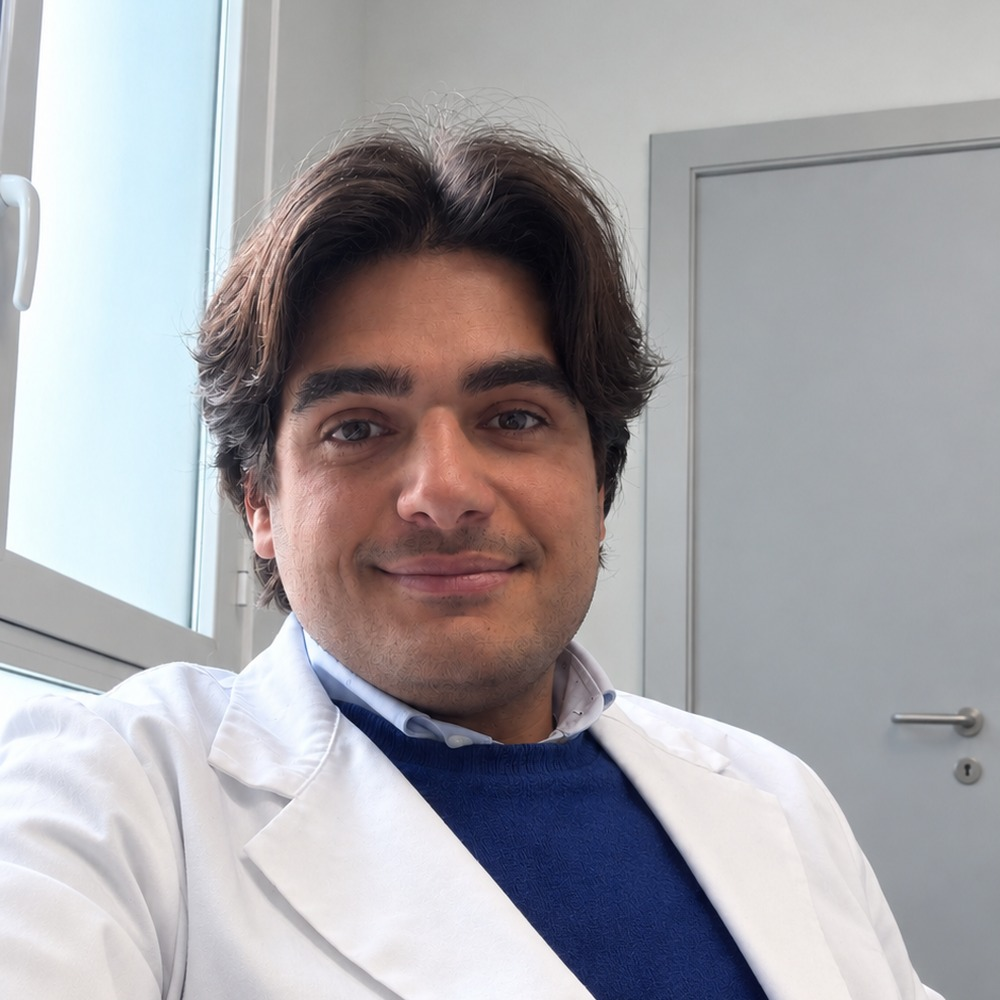
\includegraphics[width=3cm]{sagoma.jpeg} \\ \medskip

  \href{tel:+393281639295}{{\color{gray}{\faPhone}} +39 328 163 9295} \quad
  \href{mailto:simone.tringali.96@gmail.com}{{\color{gray}{\faEnvelope}} simone.tringali.96@gmail.com} \quad
  {\color{gray}{\faHome}} Italia \\ \smallskip
  {\color{gray}{\faCalendar*}} 02/02/1996 \quad
  {\color{gray}{\faCar}} Patente B
\end{center}

%====== BANNER END ======


\section{Chi sono}
%==========
\noindent \textbf{Tecnologo Alimentare} con Laurea Magistrale in \textbf{Scienze della Nutrizione Umana}, con l'obiettivo di diventare \textbf{nutrizionista}. Unisco competenze in \textbf{qualità e sicurezza degli alimenti} e \textbf{tecnologie alimentari} a una formazione in \textbf{nutrizione clinica}, maturata con il tirocinio in ambito \textbf{bariatrico} e \textbf{oncologico} e con una tesi su \textbf{alimentazione e sindrome del colon irritabile} (approccio \textbf{low-FODMAP}). Amo esplorare il legame tra \textbf{cibo}, \textbf{salute} e \textbf{benessere}, anche attraverso la pratica in \textbf{cucina}.

\section{Esperienze}
%==========
\subsection{Casa di Cura Macchiarella \rside{Palermo}}
\subsubsection{Tirocinante Nutrizionista \rside{Feb 2026 -- Apr 2026}}
\begin{itemize}
  \item Affiancamento della nutrizionista della clinica nelle consulenze di \textbf{Chirurgia Bariatrica} (fase pre- e post-operatoria) e di \textbf{Oncologia Medica}.
  \item Anamnesi alimentare, rilevazione antropometrica e stima della composizione corporea con \textbf{Bioimpedenziometria (BIA)}; calcolo del fabbisogno e \textbf{piani nutrizionali personalizzati}.
  \item Counseling a pazienti oncologici e valutazione dello stato nutrizionale (\textbf{MNA}), in \textbf{équipe multidisciplinare}.
\end{itemize}

\subsection{Istituto Sperimentale Zootecnico per la Sicilia \rside{Palermo}}
\subsubsection{Tirocinante Analista di Laboratorio \rside{Gen 2023 -- Feb 2023}}
\begin{itemize}
  \item Analisi del latte crudo con il sistema \textbf{Combifoss 7} (preparazione campioni, verifica della \textbf{qualità dei dati}) e controllo dei \textbf{parametri di qualità}: cellule somatiche, \textbf{chetosi}, \textbf{adulterazioni}.
\end{itemize}

\section{Istruzione}
%==========
\subsection{Università Telematica San Raffaele di Roma \rside{Roma}}
\subsubsection{Laurea Magistrale in Scienze della Nutrizione Umana \rside{2024 -- 2026}}
\begin{itemize}
  \item \textbf{Materie di indirizzo:} Nutrizione a livello dell'organismo: tessuti, organi e funzioni; La sindrome metabolica e le malattie dell'intestino; Disturbi del comportamento alimentare e del controllo ormonale; Intolleranze alimentari, immunità e farmaci; Metodologie dell'analisi nutrizionale.
\end{itemize}

\subsection{Università degli Studi di Palermo \rside{Palermo}}
\subsubsection{Laurea in Scienze e Tecnologie Agroalimentari \rside{2018 -- 2024}}
\begin{itemize}
  \item \textbf{Materie di indirizzo:} Microbiologia degli alimenti e dei prodotti fermentati; Tecnologie Alimentari; Chimica Nutraceutica e Metabolismo dei Nutrienti; Igiene e ispezione degli alimenti.
\end{itemize}

\section{Corsi}
%==========
\begin{itemize}
  \item \textbf{BIA START: conoscere e interpretare la metodica BIA} \aux{Akern Academy} \rside{2026}
  \item \textbf{Gestione degli effetti collaterali da farmaci incretino-mimetici} \aux{SIFA, FAD} \rside{2026}
  \item \textbf{Il paziente malnutrito: una sfida per il nutrizionista} \aux{SIFA, FAD} \rside{2026}
  \item \textbf{Terapia incretinica e nutrizione di precisione nell'obesità} \aux{SIFA, FAD} \rside{2026}
\end{itemize}

\section{Competenze}
%===============
\subsection{Trasversali}
\begin{itemize}
  \item Problem Solving, Creatività, Team Work, Adattabilità, Velocità di apprendimento.
\end{itemize}

\subsection{Informatiche}
\begin{itemize}
  \item Ottima conoscenza della suite Microsoft Office: \textbf{Word, PowerPoint, Excel}.
  \item Buona conoscenza dei sistemi operativi: \textbf{Windows, macOS}.
\end{itemize}

\subsection{Lingue}
\begin{itemize}
  \item \textbf{Italiano}: Madrelingua.
  \item \textbf{Inglese}: conoscenza intermedia.
\end{itemize}

\subsection{Interessi}
\noindent Appassionato di \textbf{cucina} e di \textbf{impasti}, amo gli sport di squadra come \textbf{calcio} e \textbf{padel}, che sviluppano il \textbf{lavoro di squadra}, e resto aggiornato sulle \textbf{innovazioni digitali}.




% \section{Certifications}
% %=======================
% \begin{enumerate}[label=\null, left=0pt..0pt, itemsep=0pt]
%   \item Some programming bootcamp, Location. \rside{2023}
%   \item Forbes Top 15 Procrastinators under 15. \rside{2022}
%   \item Perticipation award for attending workshop. \rside{2021}
% \end{enumerate}


% \section{Publications}
% %=====================
% \begin{enumerate}
%   \item A. Vaswani et al., “Attention is All you Need,” arXiv (Cornell University), vol. 30, pp. 5998 – 6008, Jun. 2017, [Online]. Available: \url{https://arxiv.org/pdf/1706.03762v5}
%   \item C. Darwin and J. Murray, \textit{On the origin of species by means of natural selection, or, The preservation of favoured races in the struggle for life.} 1859. doi: 10.5962/bhl.title.82303.
% \end{enumerate}


% \section{Awards}
% %===============
% \begin{description}
%   \item [2023] Some programming bootcamp, Location.
%   \item [2022] Forbes Top 15 Procrastinators under 15.
%   \item [2021] Conducted workshop on family planning by abstainance in SomePlace.
% \end{description}


% \section{Projects}
% %=================
% \subsection{Lunar Rover Project \aux{\href{https://robotics.nasa.gov/lmr/}{Link \linkicon}} \rside{2012 -- 13}}
% \begin{itemize}
%   \item LIDAR array, GPS, Variable FOV camera, Python, C/C++
%   \item Designed the rover to be modular, reconfigurable for sensor systems, handle science payloads, storage space, surplus resources, and robotics addons. % These modules shall be supported by centralized power and data ports. 
% \end{itemize}

% \subsection{Mars Rover \aux{\href{https://science.nasa.gov/mission/mars-exploration-rovers-spirit-and-opportunity/}{Project link \linkicon}} \rside{Feb 2012}}
% \begin{itemize}
%   \item Tech used, Language, Frameworks etc.
%   \item Implemented ABC feature
%   \item Optimised XYZ by 50\%
% \end{itemize}


\end{document}